\section{Bayesian Network}
\label{sec:design:bayesian-network}

Determining the correct action to trigger based on the contextual information is done using a Bayesian network. The network is illustrated in \cref{fig:design:bayesian-network:overview}. We consider there to be the following three levels in the network.

\begin{itemize}
\item The uppermost level containing the ``Gesture'', ``Room'', ``TV\_IsOn'' and ``MusicCentre\_IsPlaying'' nodes provides contextual information.
\item The middle level observes on the uppermost level to provide probabilities for each action in the system based on a subset of the information observed in the uppermost level.
\item The bottom level observes on all nodes in the middle level to provide probabilities for the actions in the system. Based on these probabilities the correct action to perform is determined.
\end{itemize}

The benefit of this structure is, that contextual information such as the performed gesture and the users position is always translated to probabilities for actions and these probabilities are independent of other contextual information that we may observe.

When the contextual information is modelled as probabilities for actions, it becomes trivial to combine all the contextual information to choose the right action to perform.

\begin{figure}[h!]
\centering
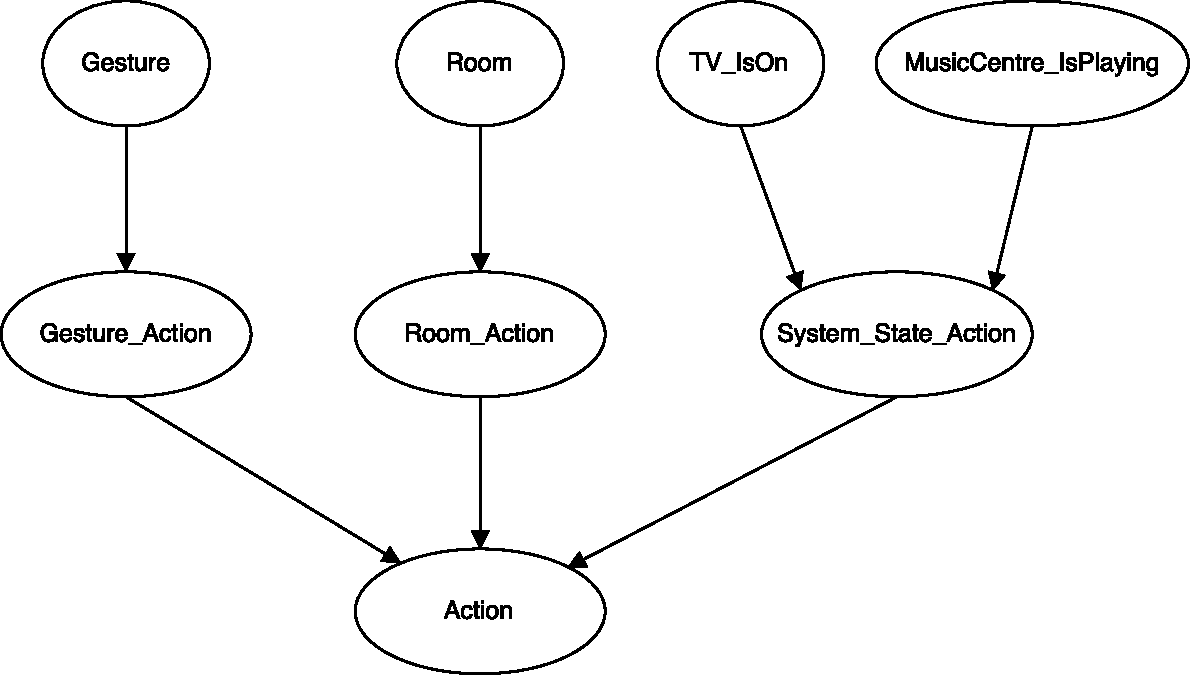
\includegraphics[width=0.75\textwidth]{images/bayesian-network}
\caption{The Bayesian network used for determining the appropriate action to trigger based on the gesture performed by the user, the position of the user and the state of the system.}
\label{fig:design:bayesian-network:overview}
\end{figure}

\begin{table}[]
\centering
\caption{Excerpt of the probability tables for the Gesture and Room nodes.}
\label{tbl:design:bayesian-network:pt-gesture-room}
\begin{tabular}{cc}
\begin{tabular}{c}
\textbf{Gesture}   \\
\begin{tabular}{ccc}
Z   & Half circle & Horizontal line \\ \hline
$\frac{1}{3}$ & $\frac{1}{3}$         & $\frac{1}{3}$
\end{tabular}
\end{tabular}
&
\begin{tabular}{c}
\textbf{Room}   \\
\begin{tabular}{ccc}
Bedroom   & Living room \\ \hline
0.5 & 0.5
\end{tabular}
\end{tabular}
\end{tabular}
\end{table}

\begin{table}[]
\centering
\caption{Probability tables for the TV\_IsOn and MusicCentre\_IsPlaying nodes.}
\label{tbl:design:bayesian-network:pt-tv-ison-musiccentre-isplaying}
\begin{tabular}{cc}
\begin{tabular}{c}
\textbf{TV\_IsOn}   \\
\begin{tabular}{cc}
Yes   & No \\ \hline
0.5 & 0.5
\end{tabular}
\end{tabular}
&
\begin{tabular}{c}
\textbf{MusicCentre\_IsPlaying}   \\
\begin{tabular}{cc}
Yes   & No \\ \hline
0.5 & 0.5
\end{tabular}
\end{tabular}

\end{tabular}
\end{table}

\begin{table}[]
\centering
\caption{Excerpt of the conditional probability table for the Gesture\_Action node.}
\label{tbl:design:bayesian-network:cpt-gesture-action}
\begin{tabular}{r|ccc}
                             & Z   & Half circle & Horizontal line \\ \hline
Lamp 3: on/off               & 0.5 & 0             & 0                \\
Lamp 8: on/off               & 0.5 & 0             & 0                \\
Music centre: next track     & 0   & 0.5             & 0                \\
Music centre: previous track & 0   & 0             & 0.5              \\
Television: next channel     & 0   & 0.5             & 0                \\
Television: previous channel & 0   & 0             & 0.5              
\end{tabular}
\end{table}

\begin{table}[]
\centering
\caption{Exceprt of the conditional probability table for the Room\_Action node.}
\label{tbl:design:bayesian-network:cpt-room-action}
\begin{tabular}{r|cc}
                             & Bedroom & Living room \\ \hline
Lamp 3: on/off               & 0 & $\frac{1}{3}$ \\
Lamp 8: on/off               & $\frac{1}{3}$ & 0 \\
Music centre: next track     & 0   & $\frac{1}{3}$ \\
Music centre: previous track & 0    & $\frac{1}{3}$ \\
Television: next channel     & $\frac{1}{3}$   & 0  \\
Television: previous channel & $\frac{1}{3}$   & 0  \\
\end{tabular}
\end{table}

\begin{table}[]
\centering
\caption{Excerpt of the conditional probability table for the System\_Action node.}
\label{tbl:design:bayesian-network:cpt-system-state-action}
\begin{tabular}{r|cc}
MusicCentre\_IsPlaying       & Yes & No \\
TV\_IsOn                     & 
\begin{tabularx}{2cm}{YY} Yes & No \end{tabularx}
&
\begin{tabularx}{2cm}{YY} Yes & No \end{tabularx}
\\ \hline
Lamp 3: on/off               & 
\begin{tabularx}{2cm}{YY} $\frac{1}{6}$ & 0.25 \end{tabularx}
&
\begin{tabularx}{2cm}{YY} 0.25 & 0.5 \end{tabularx}
\\
Lamp 8: on/off               & 
\begin{tabularx}{2cm}{YY} $\frac{1}{6}$ & 0.25 \end{tabularx}
&
\begin{tabularx}{2cm}{YY} 0.25 & 0.5 \end{tabularx}
\\
Music centre: next track               & 
\begin{tabularx}{2cm}{YY} $\frac{1}{6}$ & 0.25 \end{tabularx}
&
\begin{tabularx}{2cm}{YY} 0 & 0 \end{tabularx}
\\
Music centre: previous track               & 
\begin{tabularx}{2cm}{YY} $\frac{1}{6}$ & 0.25 \end{tabularx}
&
\begin{tabularx}{2cm}{YY} 0 & 0 \end{tabularx}
\\
Television: next channel               & 
\begin{tabularx}{2cm}{YY} $\frac{1}{6}$ & 0 \end{tabularx}
&
\begin{tabularx}{2cm}{YY} 0.25 & 0 \end{tabularx}
\\
Television: previous channel               & 
\begin{tabularx}{2cm}{YY} $\frac{1}{6}$ & 0 \end{tabularx}
&
\begin{tabularx}{2cm}{YY} 0.25 & 0 \end{tabularx}
\end{tabular}
\end{table}

%%% Local Variables:
%%% mode: latex
%%% TeX-master: "../../master"
%%% End:
